\documentclass{article}
\usepackage{graphicx} % Required for inserting images
\usepackage{graphicx} % Required for inserting images
\usepackage{float}    % For forcing figure positions
\usepackage{framed}   % For adding frames around images
\usepackage{listings} % For Java code examples
\usepackage{hyperref}

\title{Persistence Layer}

\lstset{ 
    language=Java,
    frame=single,
    basicstyle=\ttfamily,
    numbers=left,
    numberstyle=\tiny,
    breaklines=true,
    showstringspaces=false,
    captionpos=b,
    xleftmargin=\parindent,
    framexleftmargin=10pt,
    framexrightmargin=10pt,
    framextopmargin=5pt,
    framexbottommargin=5pt
}

\begin{document}

\maketitle

\section{Introduction}
The \textbf{persistence} layer acts as an intermediary between the application's business logic and the data storage systems. Its main roles include:
\begin{itemize}
    
    \item \textbf{Storing data} : It saves data generated by the application so that it can be retrieved later, even after the application is closed.

    \item \textbf{Retrieving data} : It fetches stored data when needed, allowing the application to display or manipulate this information.
    
\end{itemize}

\begin{figure}[H]
    \centering
    \begin{framed}
        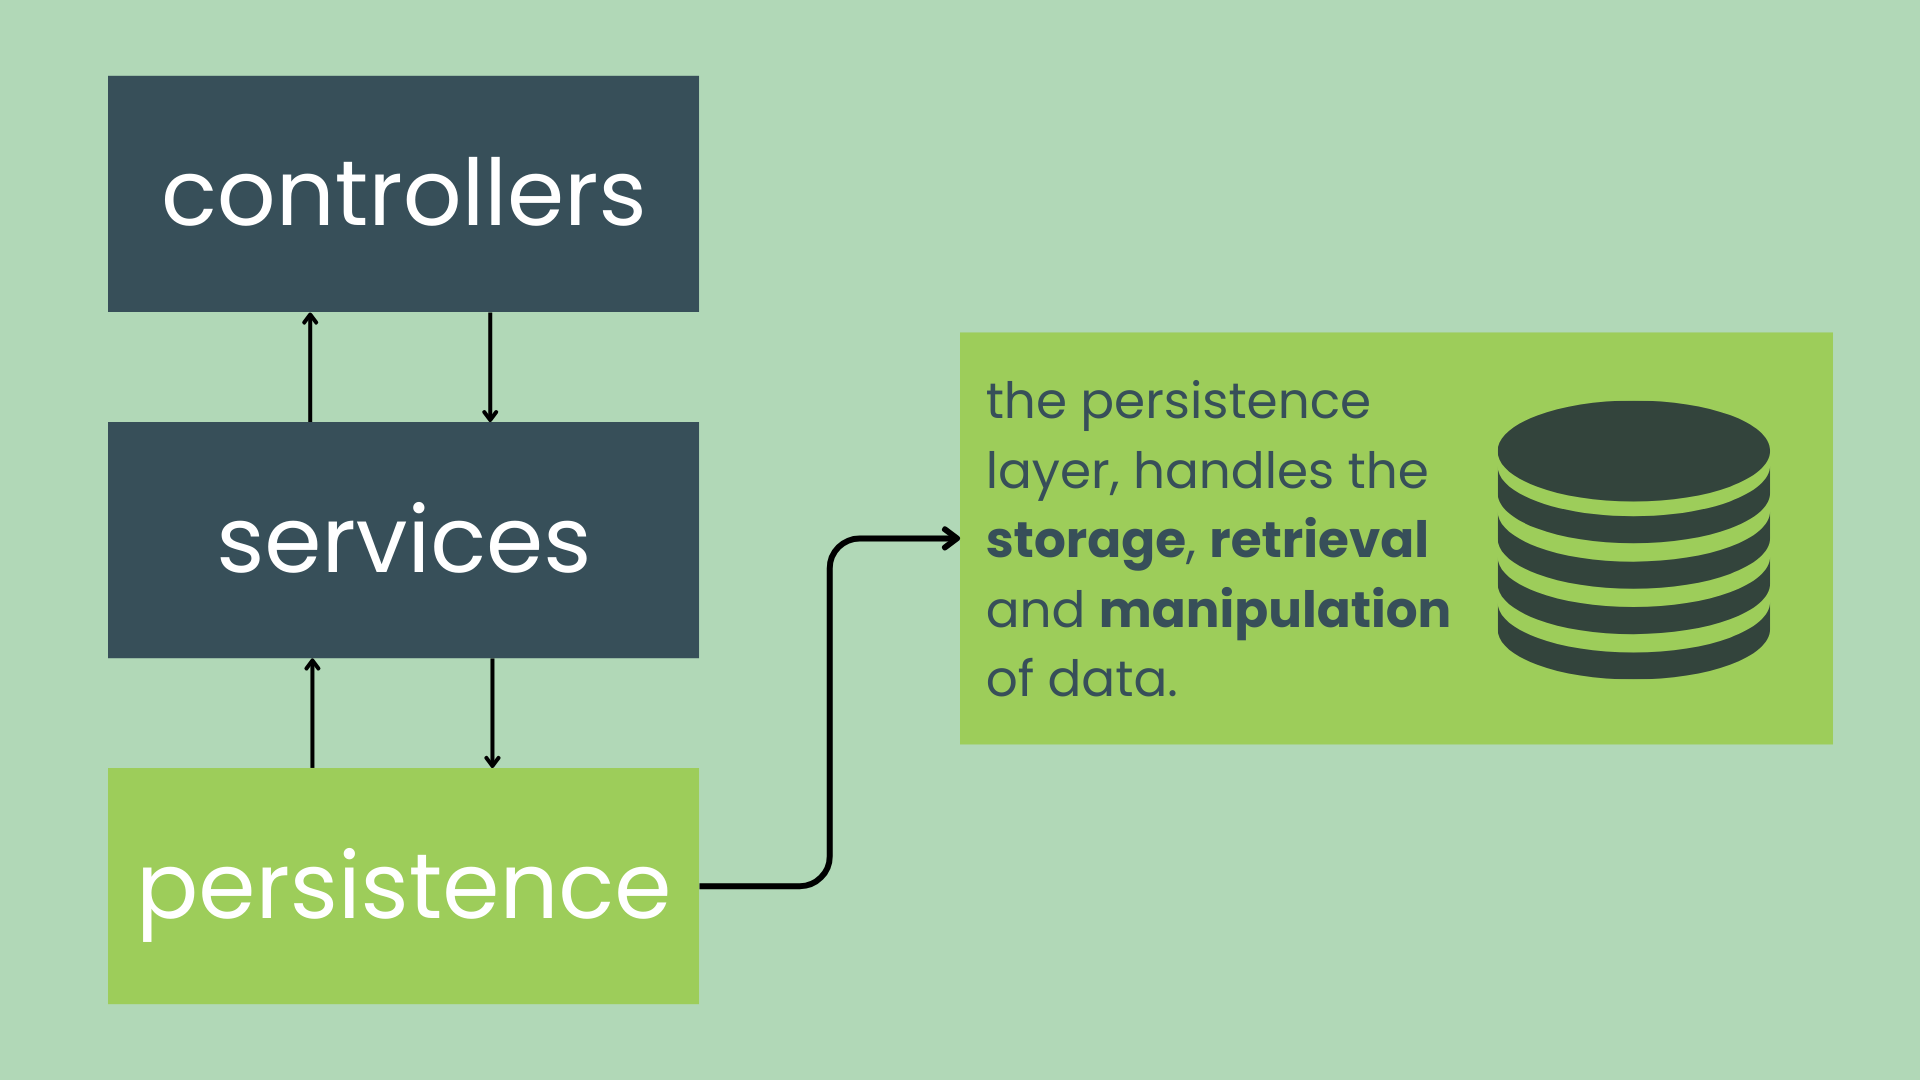
\includegraphics[width=0.8\linewidth]{images/persistence.png}
    \end{framed}
    \caption{Application layers}
    \label{fig:spring-logo}
\end{figure}

In the next sections, we are going to walk trough the different approaches to set the persistence layer up for a multi-layered application.


\section{JDBC classic approach}

\subsubsection{JDBC API}

\begin{itemize}
    \item \textbf{JDBC} (Java Database Connectivity) is an API (Application Programming Interface) that enables Java applications to interact with \textbf{relational databases}. It provides a standard set of interfaces and classes to connect to databases, execute SQL queries, and manage the results.

    \item \textbf{Low level API} : JDBC is a low-level API, meaning developers manually manage database connections, handle SQL exceptions, and close resources.

\end{itemize}

\begin{figure}[H]
    \centering
    \begin{framed}
        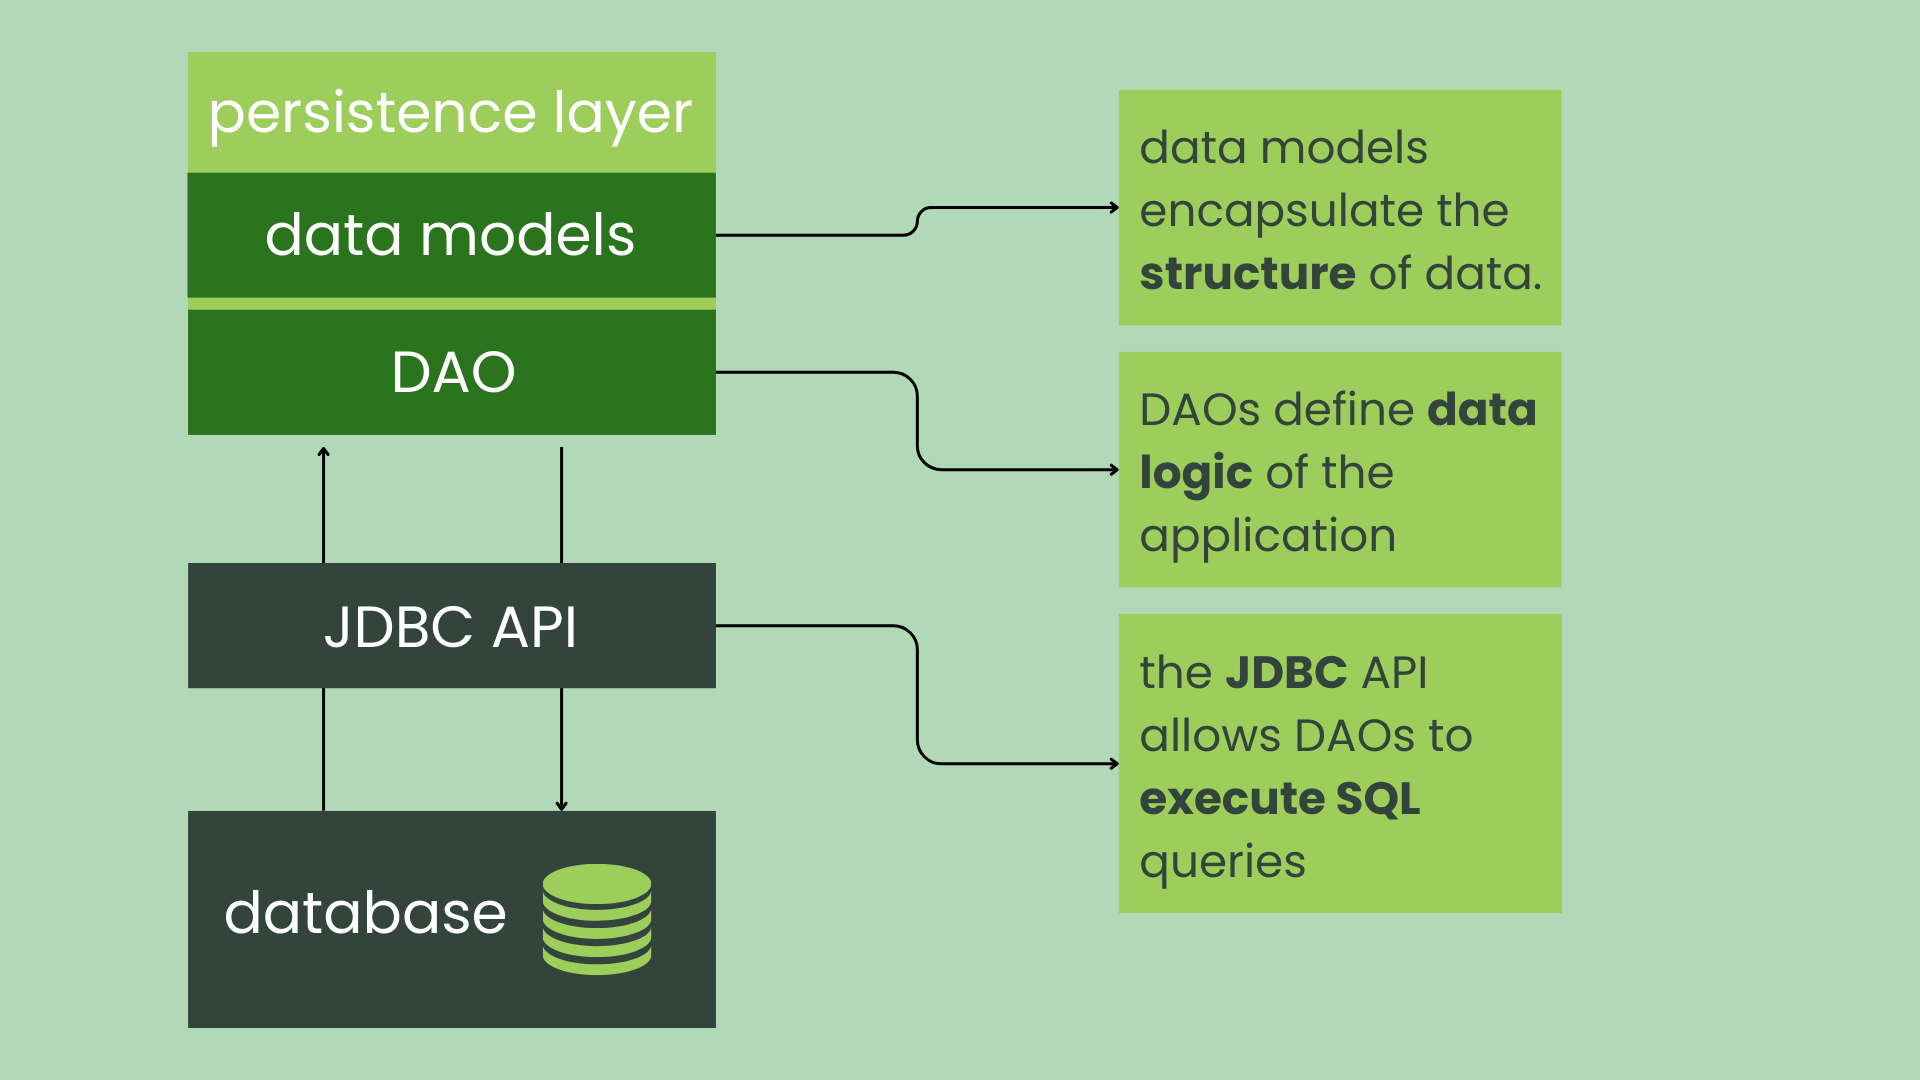
\includegraphics[width=0.8\linewidth]{images/persistence_jdbc.png}
    \end{framed}
    \caption{JDBC API}
    \label{fig:spring-logo}
\end{figure}

\subsection{Setup for the connection}

The first step in setting up the persistence layer is to include the JDBC dependency in the application classpath, either manually or by adding the appropriate Maven dependency tag. 

The architecture outlined below represents the foundation for establishing a connection in the application.

\begin{figure}[H]
    \centering
    \begin{framed}
        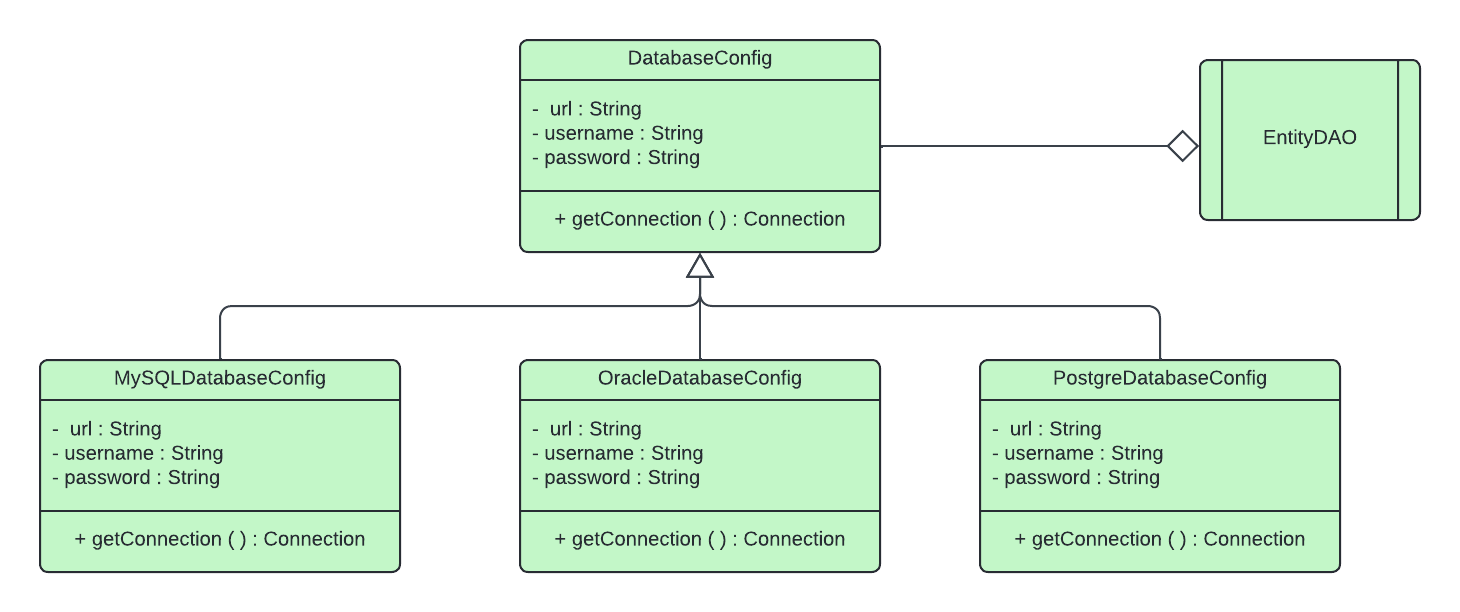
\includegraphics[width=0.8\linewidth]{images/jdbc_setup.png}
    \end{framed}
    \caption{Database Connection Setup}
    \label{fig:spring-logo}
\end{figure}


\begin{itemize}
    \item \textbf{Database Configuration}: This is an abstract class that defines the common behavior for all database configuration classes. The \texttt{getConnection()} method in this class returns the connection to the specified RDBMS.
    
    \item \textbf{Child Classes}: Each child class is responsible for establishing a connection to a specific RDBMS, inheriting from the base \texttt{DatabaseConfiguration} class.
    
    \item \textbf{DAO Class}: The DAO (Data Access Object) class handles the implementation of data logic, executing SQL queries, and using the connection provided by the database configuration class to interact with the database.
\end{itemize}

\\



\subsection{Business Data Logic}

The business data logic is built upon two core components. 

The architecture shown below outlines the general structure of the persistence layer in a \textbf{CRUD} application.

\begin{figure}[H]
    \centering
    \begin{framed}
        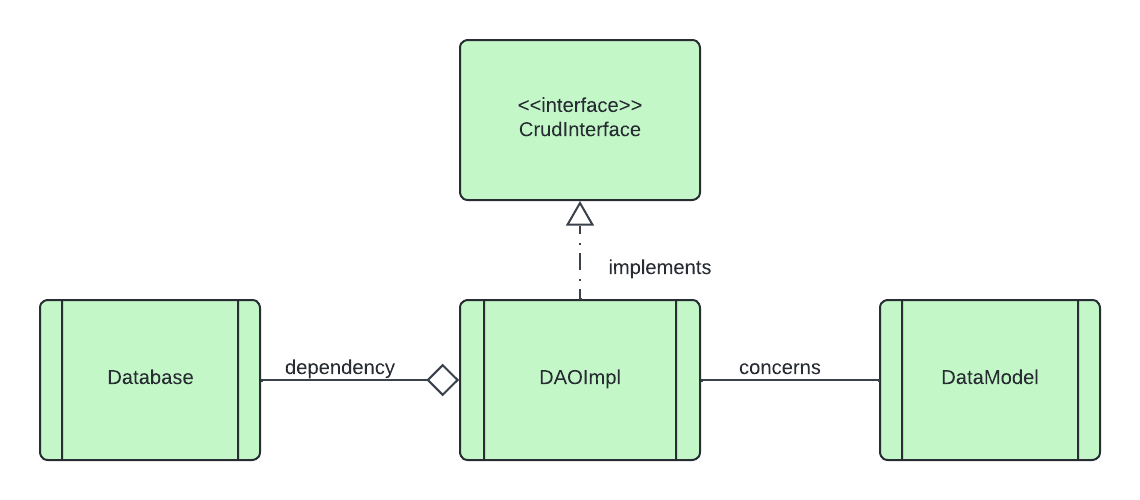
\includegraphics[width=0.8\linewidth]{images/jdbc_business_logic.png}
    \end{framed}
    \caption{Persistence Layer Architecture in a CRUD Application}
    \label{fig:spring-logo}
\end{figure}

\subsubsection*{Key Components:}

\begin{itemize}
    \item \textbf{Data Model}: A class that defines the common behavior for all concrete data model classes, representing the structure of the data that will be managed by the application.

    \item \textbf{CRUD Interface}: An interface that defines the method signatures for the core \textbf{\texttt{CRUD}} operations: Create, Read, Update, and Delete.

    \item \textbf{DAO Implementation}: Concrete classes that implement the CRUD methods for a specific data model, handling the logic for interacting with the database.
\end{itemize}

\subsection{Coding example }

Below is a simple coding example illustrating how to implement the persistence layer for a \texttt{User} entity using JDBC. This includes database configuration, a data model, a CRUD interface, and a DAO implementation. The full code is available on the project's GitHub repository:\\ \url{https://github.com/D0esN0tM1tter/spring_boot_project-/tree/master/supporting_project/persistence_examples/jdbc_classic_approach}.

\subsubsection{Database Configuration}

The \textbf{DatabaseConfiguration} class is an abstract utility class that centralizes the database connection logic. This ensures that the connection details (like URL, username, and password) are managed in one place, promoting reusability and maintainability.

\textbf{Explanation:}
\begin{itemize}
    \item \texttt{DriverManager.getConnection}: Establishes a connection to the database using the specified URL, username, and password.
    \item Constants like \texttt{URL}, \texttt{USER}, and \texttt{PASSWORD} store the configuration details securely and make them easily updatable.
    \item \texttt{Connection}: Represents an active database connection, which is necessary for executing SQL queries.
\end{itemize}

\subsubsection{User Model}

The \textbf{User} class serves as a data model to represent the structure of a record in the database. Each instance corresponds to a row in the \texttt{users} table.

\textbf{Explanation:}
\begin{itemize}
    \item Fields like \texttt{id}, \texttt{name}, and \texttt{email} map directly to the columns of the database table.
    \item Getter and setter methods allow encapsulation, enabling controlled access to these fields.
\end{itemize}

\subsubsection{CRUD Interface}

The \textbf{UserDAO} interface defines the contract for performing \textbf{CRUD} operations on the \texttt{User} data.

\textbf{Explanation:}
\begin{itemize}
    \item \texttt{createUser(User user)}: Adds a new user record to the database.
    \item \texttt{getUserById(int id)}: Fetches a user record based on its ID.
    \item \texttt{getAllUsers()}: Retrieves all user records from the database.
    \item \texttt{updateUser(User user)}: Updates an existing user record with new details.
    \item \texttt{deleteUser(int id)}: Deletes a user record based on its ID.
\end{itemize}

\subsubsection{DAO Implementation}

The \textbf{UserDAOImpl} class implements the \texttt{UserDAO} interface. It provides the concrete logic for interacting with the database.

\textbf{Explanation:}
\begin{itemize}
    \item \texttt{PreparedStatement}: Used to safely execute parameterized queries, preventing SQL injection attacks.
    \item \texttt{ResultSet}: Stores the result of \texttt{SELECT} queries, allowing iteration through the returned rows.
    \item Each method utilizes a \texttt{try-with-resources} block to ensure that connections, statements, and other resources are closed automatically.
\end{itemize}

\section{JDBC template approach}

\subsection{JDBC template} 
The Spring \textbf{JdbcTemplate} is a high-level API in the Spring Framework that simplifies database interactions by handling common tasks such as connection management, SQL statement execution, and exception handling, making data access code more concise and reducing boilerplate associated with the standard \textbf{JDBC API}.
\\
\textbf{NOTE : In order to use JDBC template, it is necessary to declare it as a dependency in the \texttt{pom.xml} file}

\begin{figure}[H]
    \centering
    \begin{framed}
        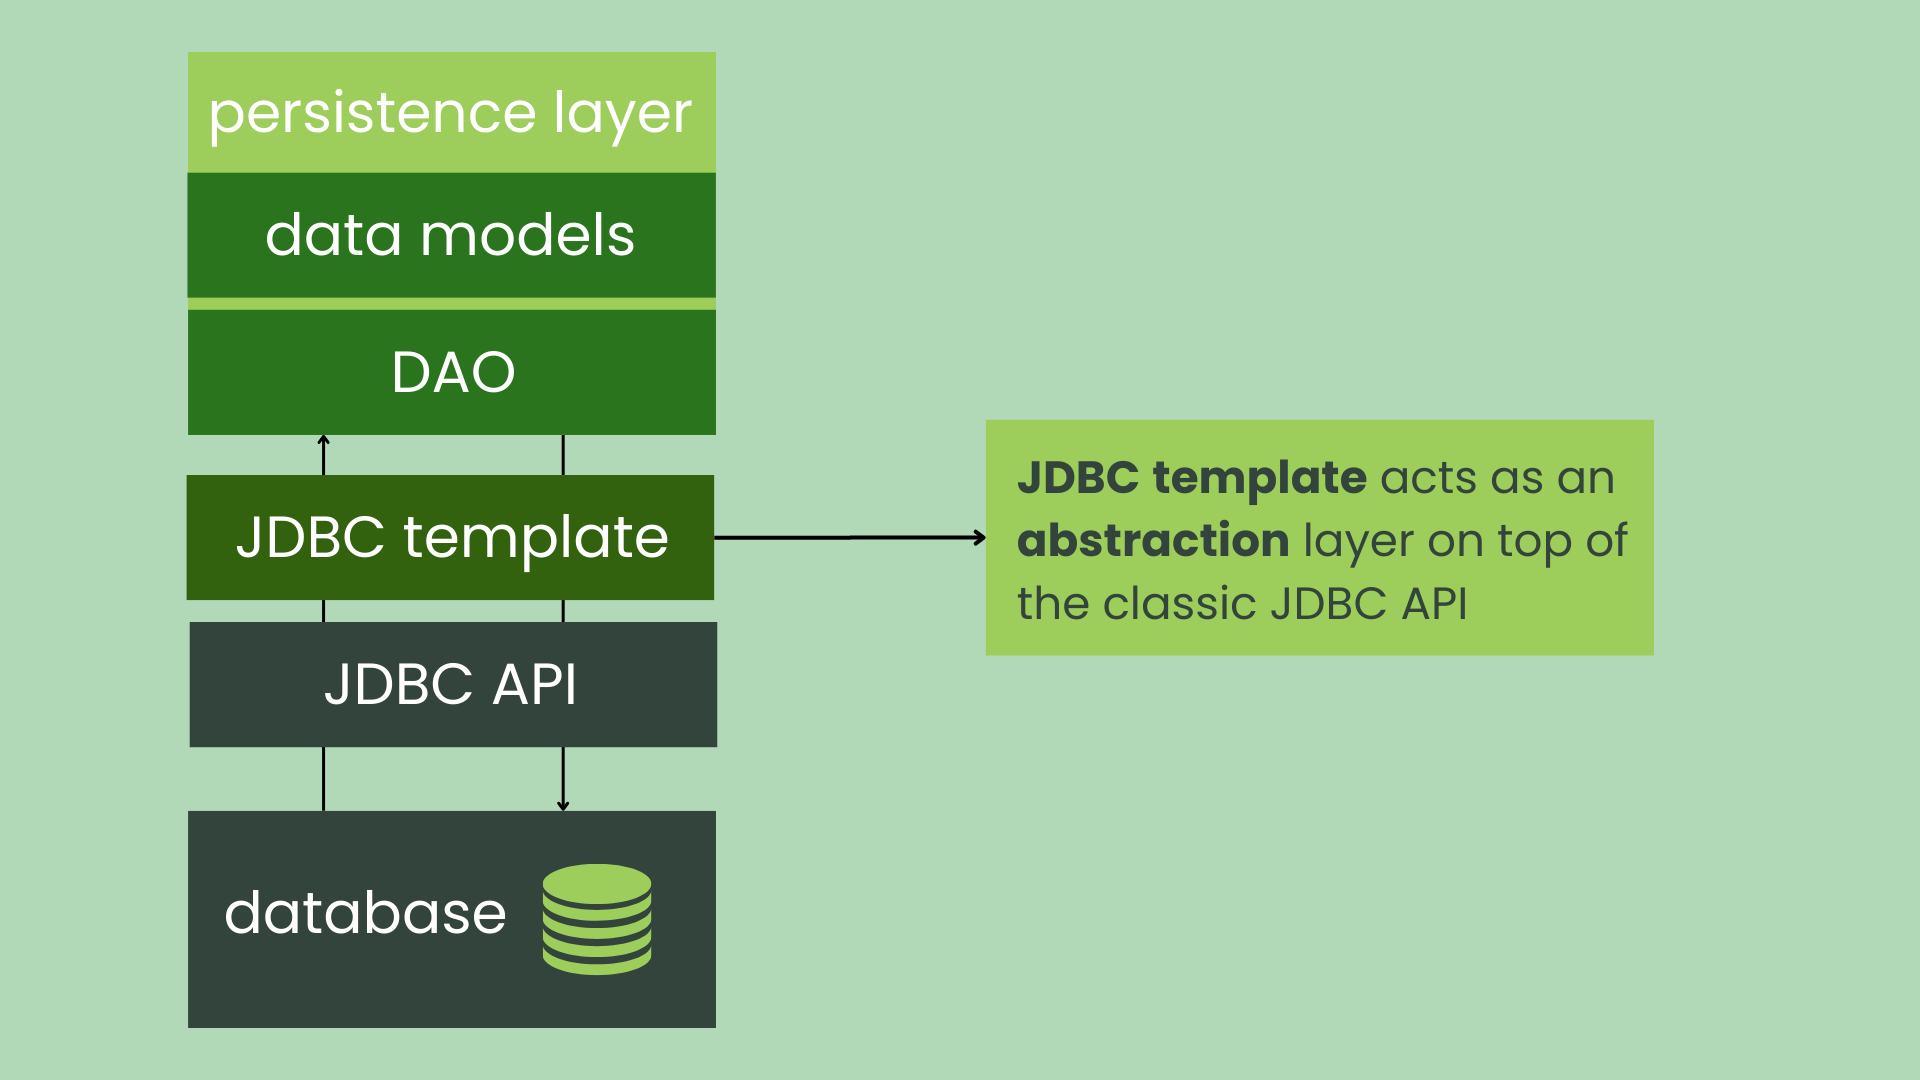
\includegraphics[width=0.8\linewidth]{images/jdbc_template.png}
    \end{framed}
    \caption{JDBC template}
    \label{fig:spring-logo}
\end{figure}

\subsection{Setup for the Connection} 
In a Spring Boot application, connection details are defined in the \textbf{\texttt{application.properties}} file. Based on this configuration, the Spring IoC (Inversion of Control) container automatically generates a \textbf{\texttt{DataSource}} object, which is then injected into the \textbf{\texttt{JdbcTemplate}} object to enable database operations.
\\
\begin{lstlisting}[caption={MySQL database configuration}]
# Database Configuration
spring.datasource.url=jdbc:mysql://localhost:3306/mydatabase
spring.datasource.username=myuser
spring.datasource.password=mypassword
spring.datasource.driver-class-name=com.mysql.cj.jdbc.Driver

\end{lstlisting}

\subsection{Data Business Logic}

In the context of using the JDBC template, the persistence layer follows an architecture similar to the previous approach. Each data model has a corresponding DAO class responsible for managing its database operations.
\\
However, instead of using \textbf{\texttt{Connection}} objects to interact with the database, DAOs now use the \textbf{\texttt{JDBC template}}.

\begin{figure}[H]
    \centering
    \begin{framed}
        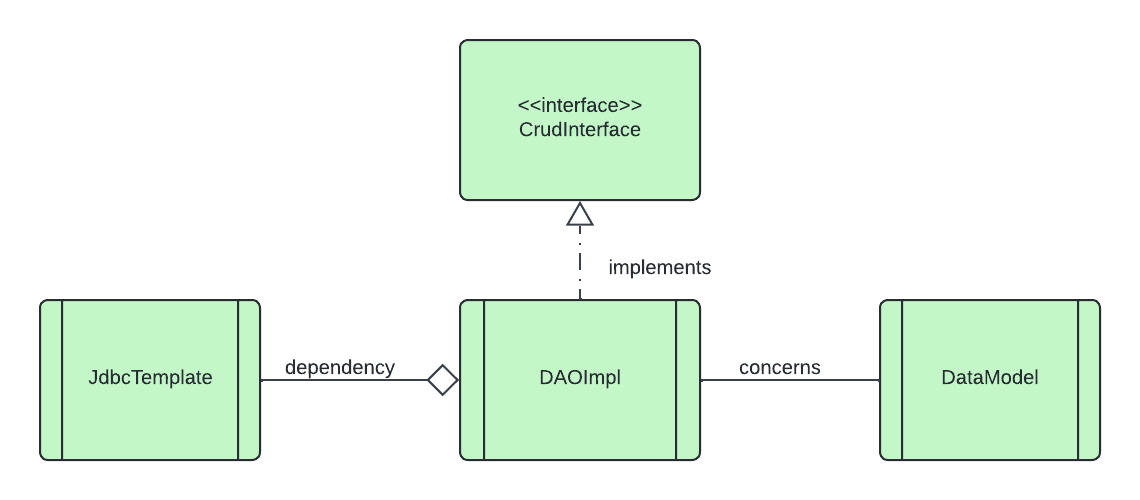
\includegraphics[width=0.8\linewidth]{images/jdbc_tem_businesslog.png}
    \end{framed}
    \caption{JDBC template}
    \label{fig:spring-logo}
\end{figure}

Setting up the persistence layer in this context involves several key steps:

\begin{enumerate}
    \item \textbf{Configuring JdbcTemplate as a Bean}: In a \textbf{\texttt{@Configuration}} class, define \texttt{JdbcTemplate} as a Spring bean. This allows the \texttt{JdbcTemplate} instance to be injected as a dependency into the DAO classes, enabling them to perform database operations.

    \item \textbf{Creating Data Models}: Define data model classes that represent the entities in the database. These classes will be used to map database records to Java objects.

    \item \textbf{Defining the CRUD Interface}: Create an interface that specifies the CRUD (Create, Read, Update, Delete) operations. This interface will be implemented by the DAOs to handle data access in a consistent way.

    \item \textbf{Implementing DAOs}: Develop DAO classes that provide concrete implementations of the CRUD operations defined in the interface. These classes will use \texttt{JdbcTemplate} to interact with the database.
\end{enumerate}

\begin{figure}[H]
    \centering
    \begin{framed}
        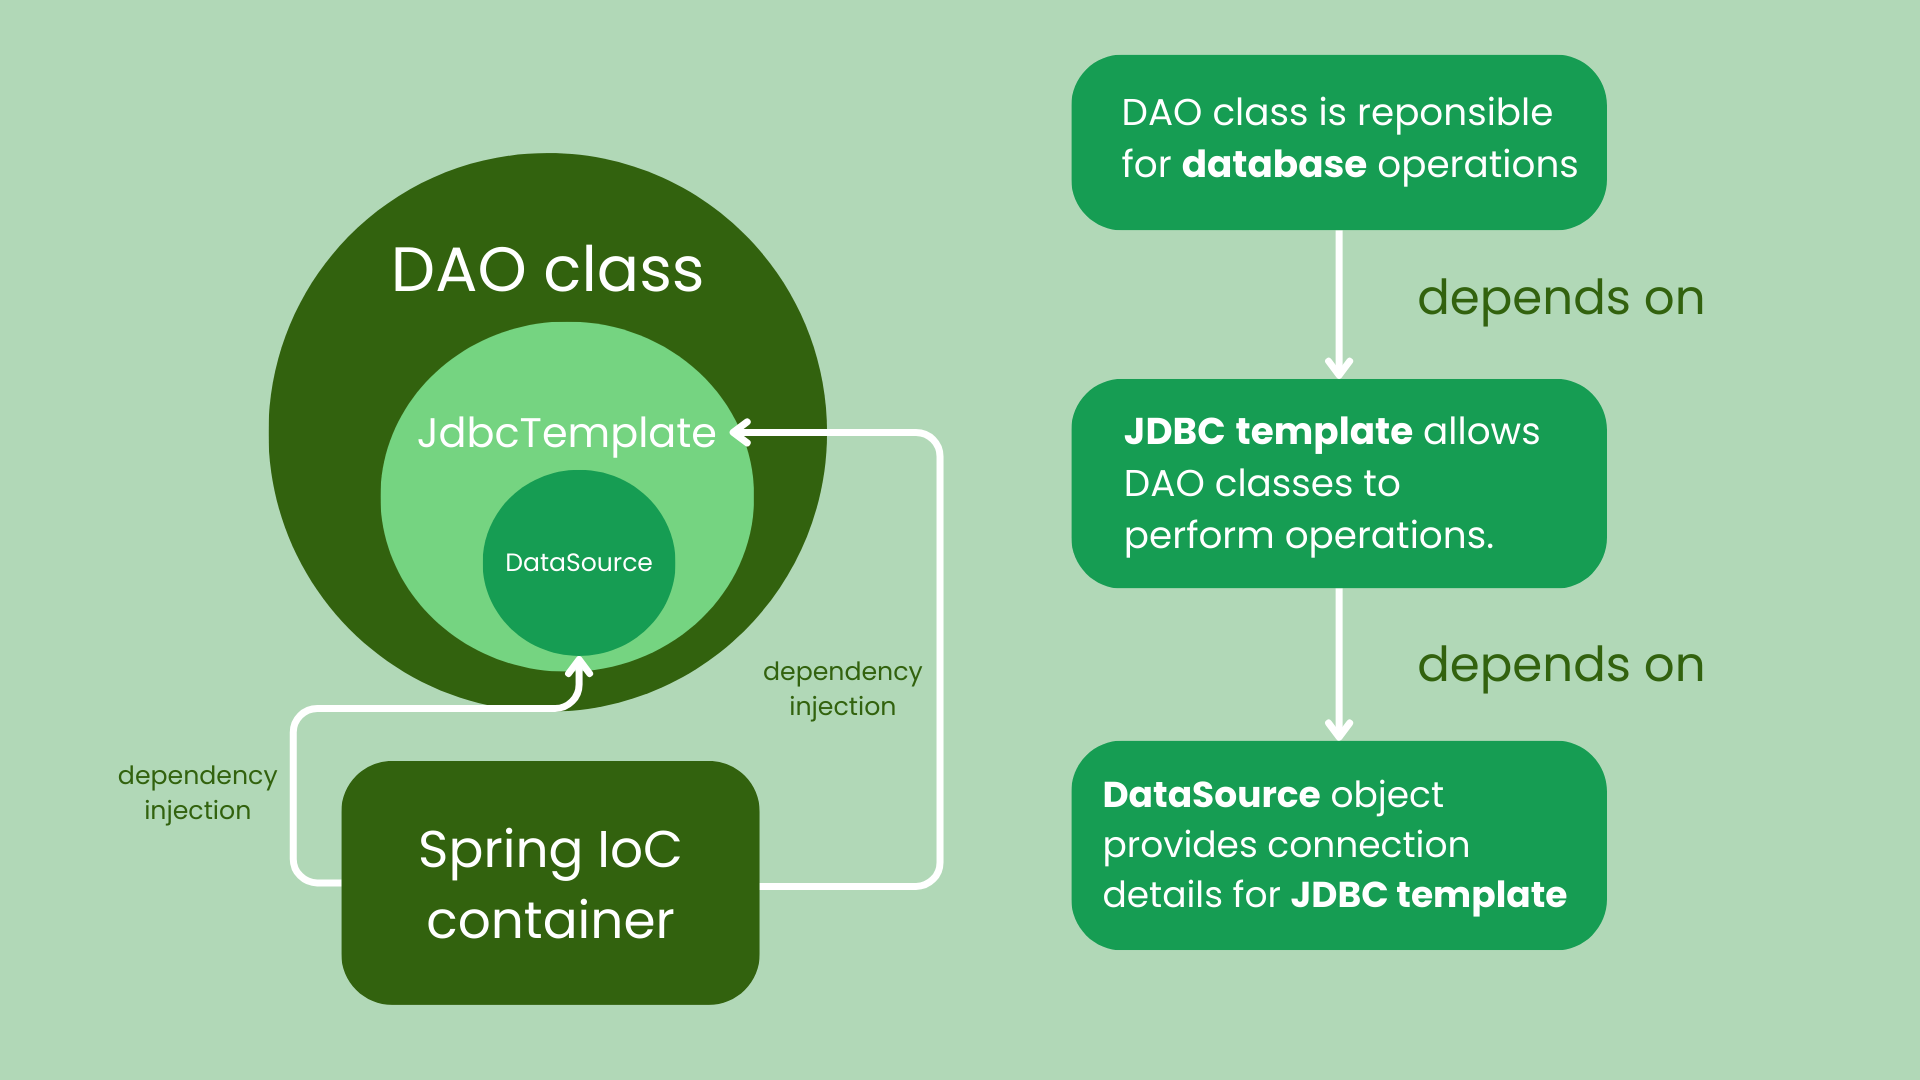
\includegraphics[width=0.8\linewidth]{images/minimalistic_jdbctemplate.png}
    \end{framed}
    \caption{Dependency Injection in the Persistence Layer}
    \label{fig:spring-logo}
\end{figure}

\subsection{Coding example}

The following example demonstrates the implementation of a persistence layer for managing a \texttt{Product} entity using Spring JDBC. It includes database configuration, a data model, a DAO interface, and a DAO implementation. The full code is available on the project's GitHub repository: \\ \url{https://github.com/D0esN0tM1tter/spring_boot_project-/tree/master/supporting_project/persistence_examples/jdbctemplate_example}.

\subsubsection{Database Configuration}

The \textbf{DatabaseConfig} class defines the \texttt{JdbcTemplate} bean, which is essential for executing SQL operations in Spring applications.

\textbf{Explanation:}
\begin{itemize}
    \item \texttt{JdbcTemplate}: A Spring-provided utility for interacting with the database in a straightforward and efficient way.
    \item \texttt{DataSource}: Injected into the \texttt{JdbcTemplate}, it provides the connection to the database.
\end{itemize}

\subsubsection{Product Data Model}

The \textbf{Product} class serves as a data model for the \texttt{Product} entity, representing a database record.

\textbf{Explanation:}
\begin{itemize}
    \item The \texttt{@Data}, \texttt{@AllArgsConstructor}, and \texttt{@NoArgsConstructor} annotations from Lombok automatically generate boilerplate code like getters, setters, and constructors.
    \item Fields like \texttt{id}, \texttt{label}, and \texttt{price} map directly to the database table's columns.
\end{itemize}

\subsubsection{Product DAO Interface}

The \textbf{ProductDao} interface defines the CRUD operations for the \texttt{Product} entity.

\textbf{Explanation:}
\begin{itemize}
    \item Methods like \texttt{save}, \texttt{update}, and \texttt{deleteById} handle the persistence logic for the \texttt{Product} entity.
    \item \texttt{findById} and \texttt{findAll} allow retrieval of one or multiple products, respectively.
\end{itemize}

\subsubsection{DAO Implementation}

The \textbf{ProductDaoImpl} class implements the \texttt{ProductDao} interface, providing concrete methods for interacting with the database.

\textbf{Explanation:}
\begin{itemize}
    \item \texttt{RowMapper}: Maps each row of the result set to a \texttt{Product} object.
    \item \texttt{KeyHolder}: Captures the auto-generated ID when a new product is inserted into the database.
    \item Each method employs \texttt{JdbcTemplate} to execute the SQL queries efficiently.
\end{itemize}

\section{Java Persistence API Approach }

This section outlines the usage of the Java Persistence API (JPA) and Hibernate for implementing a persistence layer in Java applications. It covers an introduction to JPA, the setup process for establishing a database connection, and the integration of business logic.

\subsection{JPA and Hibernate}

The Java Persistence API (JPA) is a standard specification for object-relational mapping (ORM) in Java. It provides a platform-independent approach to interact with relational databases by mapping Java objects to database tables. Hibernate is a popular JPA implementation that offers advanced ORM features and seamless integration with JPA.

\textbf{Key Features:}
\begin{itemize}
    \item Eliminates boilerplate code for managing database operations.
    \item Provides annotations for mapping Java classes to database tables.
    \item Offers a query language (JPQL) for interacting with the database in an object-oriented manner.
    \item Manages database connections and transactions automatically.
\end{itemize}

\textbf{Benefits of JPA and Hibernate:}
\begin{itemize}
    \item Simplifies database operations through entity management.
    \item Reduces the likelihood of SQL injection by using parameterized queries.
    \item Improves portability across different databases.
\end{itemize}
\subsection{Setup for the Connection}

To use JPA and Hibernate in a project, certain configurations are required to establish a connection to the database and manage entities. In a Spring Boot application, the connection and JPA settings can be configured in the \texttt{application.properties} file.

\textbf{Steps for Setup:}
\begin{enumerate}
    \item Add dependencies for JPA and Hibernate in the \texttt{pom.xml} file (Maven) or \texttt{build.gradle} file (Gradle).
    \item Create a configuration file (\texttt{application.properties}) to define database properties such as URL, username, password, and Hibernate-specific settings.
    \item Annotate Java classes with JPA annotations (\texttt{@Entity}, \texttt{@Table}, etc.) to define them as entities mapped to database tables.
    \item Use the \texttt{EntityManagerFactory} to create an \texttt{EntityManager}, which provides an interface for interacting with the persistence context.
\end{enumerate}

\textbf{Application Properties Configuration:}
To configure the MySQL database connection in a Spring Boot application, the following properties should be added to the \texttt{application.properties} file:

\textbf{Example of \texttt{application.properties} Configuration:}

\begin{lstlisting}[language=properties]
# MySQL Database Configuration
spring.datasource.url=jdbc:mysql://localhost:3306/testdb?useSSL=false&serverTimezone=UTC
spring.datasource.username=root
spring.datasource.password=
spring.datasource.driver-class-name=com.mysql.cj.jdbc.Driver
spring.jpa.database-platform=org.hibernate.dialect.MySQL5InnoDBDialect
spring.jpa.hibernate.ddl-auto=update
spring.jpa.show-sql=true
spring.jpa.properties.hibernate.format_sql=true
\end{lstlisting}

This configuration ensures that Spring Boot uses Hibernate as the JPA provider and establishes the connection to the MySQL database with the necessary credentials and settings.

\subsection{Data Business Logic}

The business logic layer interacts with the persistence layer to perform CRUD operations and apply business rules.

\textbf{Responsibilities of the Business Logic Layer:}
\begin{itemize}
    \item Validating and transforming data before persistence.
    \item Coordinating between the persistence layer and other layers of the application (e.g., controllers).
    \item Managing database transactions, ensuring data consistency.
    \item Abstracting the persistence logic from the presentation layer.
\end{itemize}

\textbf{Using Repositories:}
Repositories in JPA are interfaces that allow you to define and manage database interactions with minimal boilerplate code. Hibernate can extend these repositories to provide custom queries and advanced features.

\textbf{Entity Lifecycle Management:}
JPA provides different states for entities such as \textit{transient}, \textit{persistent}, and \textit{detached}, allowing developers to manage the entity's lifecycle effectively.

\subsection{Coding Example}
In this section, we will walk through a simple example demonstrating how to set up and use JPA with Hibernate in a Spring Boot application. The full code is available on the project's GitHub repository:\\ \url{https://github.com/D0esN0tM1tter/spring_boot_project-/tree/master/supporting_project/persistence_examples/jpa_examples}.
\vspace{0.5cm}\\
\textbf{Step 1: Entity Class}

To define a JPA entity, we need to annotate the class with \texttt{@Entity} and map it to a table in the database using \texttt{@Table}. Additionally, we use \texttt{@Id} to mark the primary key field and \texttt{@GeneratedValue} for automatic generation of the ID.

\textbf{Explanation:}
\begin{itemize}
    \item \texttt{@Entity}: Marks the class as a JPA entity.
    \item \texttt{@Id}: Specifies the primary key of the entity.
    \item \texttt{@GeneratedValue}: Configures the strategy for generating the primary key (e.g., \texttt{IDENTITY} for auto-incremented IDs).
    \item \texttt{@Column}: Maps the fields to the database columns, with options like \texttt{nullable} to define column constraints.
\end{itemize}

\subsubsection{Product Repository}

The repository interface extends \texttt{JpaRepository}, providing built-in CRUD operations.

\textbf{Explanation:}
\begin{itemize}
    \item \texttt{JpaRepository}: Provides methods like \texttt{save()}, \texttt{findById()}, \texttt{findAll()}, and \texttt{deleteById()} for database operations without needing custom implementations.
    \item Custom query methods can be added if needed.
\end{itemize}

\subsubsection{Service Layer}

The service layer interacts with the repository to handle business logic.

\textbf{Explanation:}
\begin{itemize}
    \item The service layer is used to abstract the business logic, making the controller layer cleaner.
    \item The \texttt{@Autowired} annotation injects the repository, allowing easy dependency injection.
    \item Methods like \texttt{saveProduct()} and \texttt{getProductById()} provide access to the repository’s methods for creating, retrieving, and deleting products.
\end{itemize}

\subsubsection{Controller Layer}

The controller exposes the service methods via RESTful endpoints for front-end interaction.

\textbf{Explanation:}
\begin{itemize}
    \item \texttt{@RestController}: Marks the class as a REST controller that handles HTTP requests.
    \item \texttt{@RequestMapping}: Specifies the base URL for the controller’s endpoints.
    \item \texttt{@PostMapping}, \texttt{@GetMapping}, and \texttt{@DeleteMapping}: Handle HTTP POST, GET, and DELETE requests respectively.
    \item \texttt{@RequestBody} and \texttt{@PathVariable}: Handle request payloads and dynamic URL parameters.
\end{itemize}

\textbf{Step 5: Application Configuration}

Ensure that the application is properly configured to run a Spring Boot JPA application. The configuration details can be set in the \texttt{application.properties} file, as described in the previous section.

This setup creates a complete flow for managing entities in a Spring Boot application with JPA and Hibernate. With minimal configuration, Spring Boot handles most of the boilerplate code, allowing developers to focus on business logic.



\section{Conclusion}

In this chapter, we explored different approaches for managing the persistence layer in a Spring Boot application. We covered the implementation of persistence with JDBC, detailing the database configuration, data models, and CRUD interfaces, as well as using \texttt{JdbcTemplate} to interact with the database. In parallel, we also discussed setting up persistence with JPA and Hibernate, configuring the database connection, and defining entities using JPA annotations. These two approaches offer different advantages depending on the project's needs: JDBC for more manual and controlled operations, and JPA/Hibernate for automated management and simplified object-relational mapping. By combining these techniques, we can build a robust, flexible, and maintainable persistence layer.

\end{document}
